%!TEX encoding=UTF-8
%!TEX program=xelatex
\documentclass[pre,twocolumn]{revtex4-2}
\usepackage{amsmath}
\usepackage{amssymb}
\usepackage{xeCJK}
\usepackage{graphicx}
\usepackage{float}
\usepackage{braket}
\usepackage{algpseudocode}
\DeclareMathOperator*{\argmax}{arg\,max}

\renewcommand{\textfraction}{0.05}
\renewcommand{\topfraction}{0.95}
\renewcommand{\bottomfraction}{0.95}
\renewcommand{\floatpagefraction}{0.85}
\renewcommand{\dbltopfraction}{0.95}
\renewcommand{\dblfloatpagefraction}{0.85}

\setCJKmainfont{SimSun}
\setCJKmonofont{SimHei}

\begin{document}

\title{连续时间量子游走辅助贪心算法面向最大团问题的量子启发式图优化实验}

\author{任子桐}
\author{司浩言}
\author{许适丞}
\author{朱鑫池}
\affiliation{浙江大学竺可桢学院，杭州}

\date{\today}

\begin{abstract}
本项目验证使用连续时间量子游走（CTQW）辅助经典贪心算法求解最大团问题的可行性。针对经典贪心易陷入局部最优、难以感知全局拓扑的痛点，提出“量子全局 + 经典局部”的混合架构：通过引入种子扰动项的哈密顿量使量子概率分布感知当前搜索状态，并与经典评分融合。实验表明：CTQW 具备识别图全局团结构的能力（团节点概率约为背景的 $7$ 倍）；但将 CTQW 嵌入贪心内部时，每轮不稳定的局部扩散会污染原本稳健的经典判断，反而不及经典基线；而将量子游走改作贪心外部的起点选择器，则能在统计上显著超越经典强基线。进一步在大规模人工与 DIMACS 真实数据集上、对嵌入式与外置式（含 Krylov 与 Chebyshev 两种近似）方案做了效率与准确度测试，发现外置式 Krylov 近似在真实数据集上的准确度有反超经典算法的趋势。本研究证实量子动力学机制在启发式算法设计中具有实际价值。
\end{abstract}

\maketitle

\section{简介}

\subsection{问题背景}
最大团问题（Maximum Clique Problem, MCP）是图论中最经典的 NP-Hard 组合优化问题之一：给定无向图 $G=(V,E)$，要求找出一个节点集合 $S\subseteq V$，使得 $S$ 中任意两点均有边相连（即 $S$ 为一个团），且 $|S|$ 达到最大。该问题在社交网络中的社区发现、生物信息学中的蛋白质相互作用网络分析、计算化学中的分子相似性匹配、物流与调度等场景中均有重要应用~\cite{pardalos1994}。然而由于其计算复杂度极高、目前不存在多项式时间精确解法，当图规模稍大（数百节点以上）便难以求得精确解。实际工程中通常采用基于度数的贪心算法、局部搜索或模拟退火~\cite{kirkpatrick1983}等启发式方法进行近似求解。

传统贪心算法从一个起点出发，每一轮依据节点的度数等局部指标在候选集合中选择下一个节点：这种"局部最优 $\Rightarrow$ 全局近似"的策略实现简单、速度快，但有两个根本性缺陷。其一，**局部最优陷阱**：贪心一旦选错一个度数高但远离真正团结构的"诱饵节点"，后续无法回溯；其二，**全局拓扑盲区**：度数等局部统计量只反映节点的一阶邻接信息，无法感知图中长程的多步路径与子结构密度。这两个缺陷决定了纯经典贪心难以在复杂拓扑下逼近最优解，亟需引入具有全局视野的辅助信号。

\subsection{量子游走与本项目动机}
连续时间量子游走（Continuous-Time Quantum Walk, CTQW）最早由 Farhi 和 Gutmann 于 1998 年提出~\cite{farhi1998}，作为经典连续时间随机游走的量子对应：经典随机游走描述概率分布在图上的扩散，CTQW 描述概率幅在图上的相干演化。Childs 等人在后续工作中证明 CTQW 在某些"焊接树"图上对经典算法存在指数级搜索加速~\cite{childs2009}，确立了量子游走在图算法领域的理论价值。直观上，CTQW 的优势来源于矩阵指数 $e^{-iHt}$ 中相干叠加的多步路径贡献——经典随机游走只看一步邻接，而 CTQW 在演化中"同时感知"了所有长度的路径，因此在原理上具备识别图全局拓扑的能力。

将这一能力嫁接到组合优化是近年来的活跃研究方向，但既有工作多聚焦于纯量子算法（如 QAOA、量子退火），将量子动力学作为\emph{启发式信号}与经典算法\emph{混合}使用的工作仍较少。本项目的核心动机正在于此：验证 CTQW 产生的节点概率分布能否作为一种有效的全局结构信号，辅助经典贪心算法突破局部最优。我们不追求"完全量子化"的算法，而是探索"量子全局 + 经典局部"的混合架构，并以最大团问题作为具体落脚点。这一研究思路的价值在于：(i)~量子算法在 NISQ（含噪中等规模量子）时代真正落地的途径之一就是与经典算法混合；(ii)~量子信号到底应该\emph{如何接入}经典流程，是一个尚未被充分研究的工程问题，本项目通过设计两种截然不同的接入方式（嵌入式 vs 外置式）为这一问题提供实证答案。

\section{模型与方法}

\subsection{连续时间量子游走模型}
CTQW 是经典随机游走的量子对应：经典随机游走描述概率分布在图上的扩散，CTQW 则描述概率幅在图上的相干演化。在图 $G=(V,E)$ 上，以节点基态 $\ket{v}$ 张成系统状态 $\ket{\psi(t)}=\sum_{v\in V}\alpha_v(t)\ket{v}$，节点 $v$ 被观测到的概率为 $P_v(t)=|\alpha_v(t)|^2$。演化由薛定谔方程给出（取 $\hbar=1$）：
\begin{equation}
i\frac{\partial}{\partial t}\ket{\psi(t)}=H\ket{\psi(t)},
\end{equation}
其形式解为 $\ket{\psi(t)}=U(t)\ket{\psi_0}$，演化算子 $U(t)=e^{-iHt}$。于是
\begin{equation}
P_v(t)=|\braket{v|e^{-iHt}|\psi_0}|^2.
\label{eq:prob}
\end{equation}
若 $H$ 为 Hermitian 矩阵，则 $U(t)$ 幺正，$U^\dagger U=I$，状态范数守恒，故 $\sum_{v\in V}P_v(t)=1$，$P_v(t)$ 是一个合法的节点概率分布。

CTQW 概率能反映全局拓扑的数学原因在于矩阵指数的展开 $e^{-iHt}=I-iHt-\tfrac{H^2t^2}{2!}+\cdots$：当 $H=A$ 时，$(A^k)_{uv}$ 与图中 $u\to v$ 长度为 $k$ 的路径数相关，因此演化综合了不同长度路径对概率幅的贡献，而不只是单个节点的度数。

\subsection{哈密顿量设计：候选解引导演化}
若直接取 $H=A$，CTQW 只反映原图结构，无法利用贪心已选出的中间解。为使量子演化与搜索状态相关，引入种子集合 $S\subseteq V$ 的扰动项：
\begin{equation}
H=A+\lambda\sum_{u\in S}\ket{u}\bra{u},
\label{eq:ham}
\end{equation}
其中 $\lambda$ 为扰动强度，$\ket{u}\bra{u}$ 是仅第 $u$ 个对角元为 $1$ 的投影算子。该项相当于对已选节点施加与搜索状态相关的局域势，使第 $r$ 轮的哈密顿量 $H^{(r)}=A+\lambda\sum_{u\in S^{(r)}}\ket{u}\bra{u}$ 随部分解动态变化。$\lambda$ 是关键参数：过小则退化为只看原图结构，过大则概率过度集中于种子附近、削弱探索能力，其合理区间需由实验确定（取 $\lambda\in\{0,0.1,0.5,1,2,5\}$）。

\subsection{初始态设计}
为与当前贪心状态结合，采用基于种子集合的均匀初态
\begin{equation}
\ket{\psi_0}=\frac{1}{\sqrt{|S|}}\sum_{u\in S}\ket{u},
\end{equation}
其归一化由基态正交性保证。当 $S=\varnothing$ 时，可选用全图均匀初态 $\ket{\psi_0}=\frac{1}{\sqrt{|V|}}\sum_{v\in V}\ket{v}$（无先验偏置，从全图出发）或以最高度节点 $s_0=\arg\max_v\deg(v)$ 为种子的经典启发式初始化。两种初态对应 CTQW 的两种物理模式，是后文区分嵌入式与外置式方案的关键。

\subsection{候选集合约束}
量子概率不能直接决定选择，因为问题本身有约束。对最大团任务，候选节点必须与 $S$ 中所有节点相连：
\begin{equation}
C(S)=\{v\in V\setminus S\mid \forall u\in S,\ (u,v)\in E\}.
\end{equation}
由归纳法易证：只要每轮都从 $C(S)$ 中选点，输出集合始终是合法团；当 $C(S)=\varnothing$ 时算法停止。候选集合相当于先做“可行性投影”，再让评分参与排序。

\subsection{评分函数设计}
设计三类评分以支持对照与消融。\textbf{经典评分}：因最大团任务中所有合法候选都满足简单连接比例为 $1$、无法区分，故采用候选诱导子图度数 $R_{\mathrm{clique}}(v,S)=\deg_{C(S)}(v)$，衡量选择 $v$ 后团的可扩展性。\textbf{量子评分}：$Q(v,S)=P_v(t)$，仅在候选集合上比较。\textbf{混合评分}：
\begin{equation}
\mathrm{Score}(v,S)=\alpha\,\widetilde{Q}(v,S)+(1-\alpha)\,\widetilde{R}(v,S),
\label{eq:score}
\end{equation}
其中 $\widetilde{Q},\widetilde{R}$ 为在 $C(S)$ 上做 min-max 归一化后的评分，$\alpha\in\{0,0.25,0.5,0.75,1\}$ 控制量子—经典权衡（$\alpha=0$ 纯经典，$\alpha=1$ 纯量子）。归一化是必要的，因为 $Q$ 是 $[0,1]$ 概率而 $R$ 是整数度数，尺度不同会使 $\alpha$ 失去清晰含义。图~\ref{fig:framework} 给出候选集合与评分融合框架。

\begin{figure}[H]
\centering
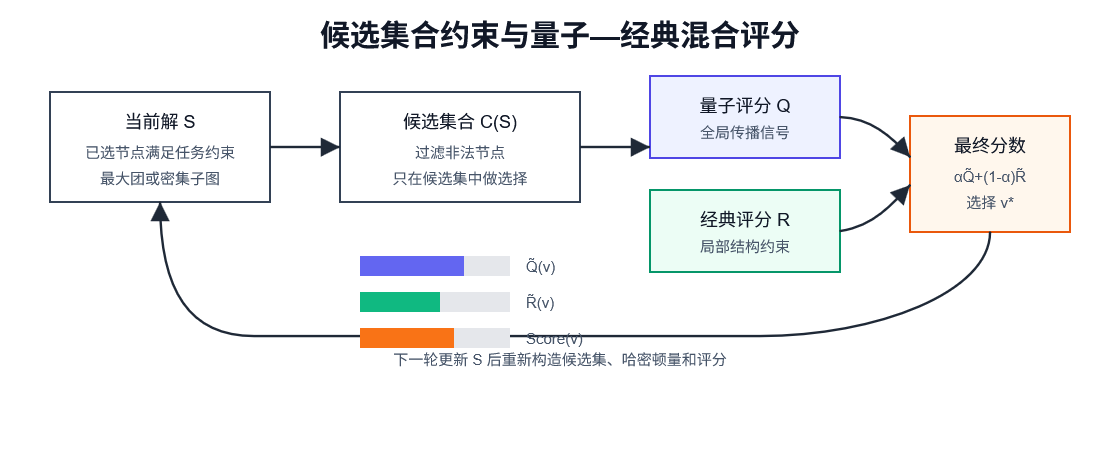
\includegraphics[width=7.5cm]{figures/framework.png}
\caption{候选集合与评分融合框架：候选集合保证“选出的节点合法”，混合评分决定“合法节点中哪个更值得选”。}
\label{fig:framework}
\end{figure}

\subsection{一轮决策示例}
以图~\ref{fig:example} 的 $7$ 节点图为例（$\{1,2,3,4\}$ 构成 4-团）。设已选 $S=\{1,2\}$，则候选集合 $C(S)=\{3,4,5\}$。构造 $H=A+\lambda(\ket{1}\bra{1}+\ket{2}\bra{2})$、$\ket{\psi_0}=\frac{1}{\sqrt2}(\ket{1}+\ket{2})$，取 $\lambda=t=1$。设本轮 CTQW 概率为 $Q(3)=0.31,Q(4)=0.24,Q(5)=0.18$；候选子图度数 $R(3)=2,R(4)=R(5)=1$。归一化并取 $\alpha=0.5$ 后的混合评分见表~\ref{tbl:example}，本轮选择 $v^*=3$，更新 $S\leftarrow\{1,2,3\}$。该例展示：候选集合先排除非法节点，$Q$ 反映传播关系，$R$ 避免选到扩展性差的节点，且每轮更新 $S$ 后哈密顿量、初始态、评分都随之改变——算法是动态迭代而非一次性静态排序。

\begin{figure}[H]
\centering
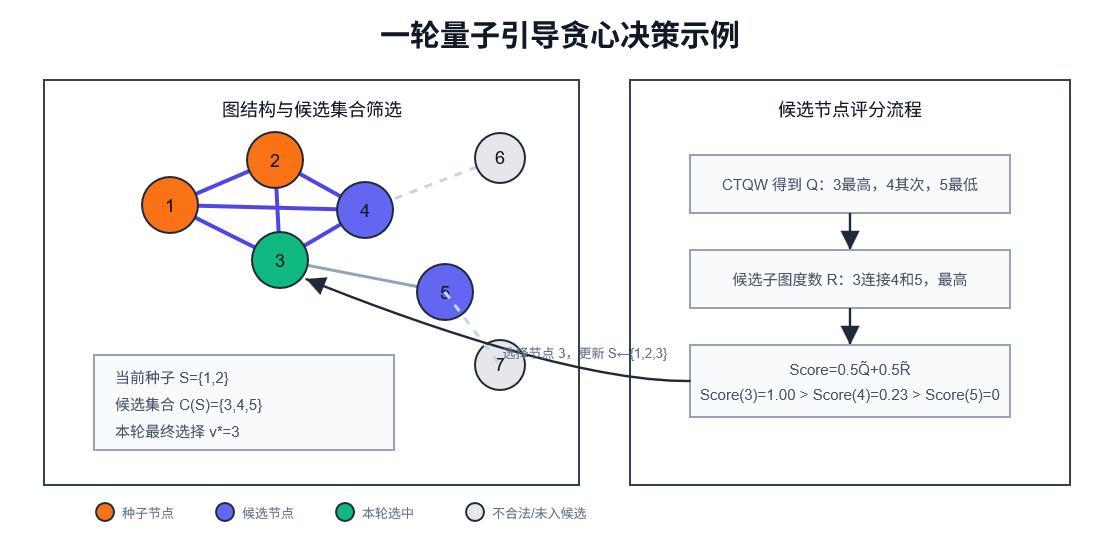
\includegraphics[width=6.5cm]{figures/decision_example.png}
\caption{一轮决策示例图，$\{1,2,3,4\}$ 构成一个 4-阶团。}
\label{fig:example}
\end{figure}

\begin{table}[H]
\caption{候选节点评分计算示例（$\alpha=0.5$）。}
\label{tbl:example}
\centering
\begin{tabular}{cccc}
\hline\hline
候选 $v$ & $Q(v,S)$ & $R(v,S)$ & 混合评分 \\
\hline
3 & 0.31 & 2 & 1.00 \\
4 & 0.24 & 1 & 0.23 \\
5 & 0.18 & 1 & 0.00 \\
\hline\hline
\end{tabular}
\end{table}

\subsection{算法流程}
量子引导贪心算法的伪代码如下：

\par\vspace{1ex}\noindent\rule{\columnwidth}{0.8pt}\par\vspace{-0.3ex}
\noindent\textbf{Algorithm 1}\quad Quantum-guided Greedy for Maximum Clique
\par\vspace{-0.3ex}\noindent\rule{\columnwidth}{0.4pt}\par\vspace{0.3ex}
\begin{algorithmic}[1]
\Require Graph $G=(V,E)$ with adjacency matrix $A$; evolution time $t$; perturbation strength $\lambda$; balance coefficient $\alpha$.
\Ensure Clique node set $S$.
\State Initialize seed set $S$
\While{stopping condition not met}
    \State Compute candidate set $C(S)$
    \If{$C(S) = \varnothing$}
        \State \textbf{break}
    \EndIf
    \State $H \gets A + \lambda \sum_{u \in S}\ket{u}\bra{u}$ \Comment{Seed-perturbed Hamiltonian}
    \State $\ket{\psi_0} \gets \tfrac{1}{\sqrt{|S|}}\sum_{u \in S}\ket{u}$
    \State $\ket{\psi_t} \gets e^{-iHt}\ket{\psi_0}$ \Comment{CTQW evolution}
    \For{each $v \in C(S)$}
        \State $Q(v) \gets |\braket{v|\psi_t}|^2$ \Comment{Quantum score}
        \State $R(v) \gets \deg_{C(S)}(v)$ \Comment{Classical degree score}
    \EndFor
    \State Normalize $Q,R$ on $C(S)$ to get $\widetilde{Q},\widetilde{R}$
    \State $\mathrm{Score}(v) \gets \alpha\,\widetilde{Q}(v) + (1-\alpha)\,\widetilde{R}(v)$
    \State $v^* \gets \argmax_{v \in C(S)} \mathrm{Score}(v)$
    \State $S \gets S \cup \{v^*\}$
\EndWhile
\State \Return $S$
\end{algorithmic}
\par\vspace{0.3ex}\noindent\rule{\columnwidth}{0.8pt}\par\vspace{1ex}

\subsection{方法边界}
本方法存在若干边界：CTQW 概率对 $t$、$\lambda$ 与初始态较敏感，单一参数下的好结果不能证明普遍有效；对小图有效不代表大图可扩展（矩阵指数计算可能成为瓶颈，详见实验四的近似方案）；量子概率高不等于节点必属最优解，故必须保留候选集合约束与经典评分。本项目要论证的是“CTQW 概率作为图优化启发式信号是否有用”，而非声称其在所有图上严格优于经典算法。

\section{研究问题与实验设计}

\subsection{研究问题分解}
本项目要回答的核心问题——"CTQW 的全局概率信号能否、并以何种方式辅助经典贪心解决最大团问题"——在工程上过于笼统，难以直接证伪。我们将其分解为四个层级递进、彼此独立可验证的子假设：

\noindent\textbf{H1（信号有效性）}\quad 在全图均匀初态下演化的 CTQW，团节点的概率显著高于背景节点，且该信号在度数指标之外提供独立的全局结构信息。该假设是后续一切研究的前提：如果 CTQW 概率本身就识别不出团结构，则任何接入方式都没有意义。

\noindent\textbf{H2（嵌入式融合）}\quad 把 CTQW 嵌入贪心迭代、每轮按当前部分解 $S$ 重算概率，并按式~\eqref{eq:score} 与经典度数评分加权融合后，求解质量能优于纯经典强基线。这是最直接、最符合直觉的接入方式——让量子信号参与每一步决策。

\noindent\textbf{H3（外置式接入）}\quad 若 H2 不成立，则改将 CTQW 从贪心内部移出、置于其外部专做起点选择器，仅以全图均匀初态下的概率挑选 Top-$K$ 节点作为多次贪心重启的起点，此时能在严格对照下反超经典强基线。该假设的目的是分离 CTQW 的两种使用模式（全局识别 vs 局部扩散），并诊断 H2 失败的原因。

\noindent\textbf{H4（可扩展性）}\quad 在大规模人工图与 DIMACS 真实图上，将精确矩阵指数 $e^{-iHt}$ 替换为 Krylov 子空间与 Chebyshev 多项式两种稀疏近似后，H2/H3 的结论在准确度与运行时间上仍能成立，甚至在真实数据集上呈现新的趋势。该假设面向"量子启发式算法能否走出玩具规模"这一更现实的工程问题。

四个假设的设计遵循\emph{递进证伪}原则：H1 是地基，H2/H3 是互补的两种接入方式（任何一个成立即可支撑核心结论），H4 检验工程可扩展性。无论中间结果正/负，都能为最终结论提供有效信息。

\subsection{实验—假设对应关系}
四组实验逐一对应四个假设：
\begin{itemize}
\item \textbf{实验一 $\to$ H1}：在含 planted clique 的小图上直接可视化 CTQW 概率分布，统计团内/外节点的平均概率比，并与度数信号做散点对比，定量验证 CTQW 是否提供独立的全局信号。
\item \textbf{实验二 $\to$ H2}：将完整 Algorithm 1（嵌入式量子引导贪心）与经典强基线作配对对比，并在 $\alpha\in\{0,0.25,0.5,0.75,1\}$ 上做参数扫描、在 (Q, R, $\lambda$) 三个组件上做消融实验，判断 H2 是否成立及失败原因。
\item \textbf{实验三 $\to$ H3}：基于实验二的失败诊断，设计外置式 MultiStartCTQW 方案；并引入 MultiStartRandom（剥离"多起点本身有效"）与 MultiStartDegree（剥离"任意全局信号都有效"）两组对照，确保任何性能提升只能归因于 CTQW 本身。
\item \textbf{实验四 $\to$ H4}：把嵌入式与外置式两种方案都迁移到大规模图，分别用 Krylov 与 Chebyshev 两种近似替换精确矩阵指数，在人工 large 数据集和 DIMACS 真实数据集上做效率与准确度双重测试。
\end{itemize}

\subsection{数据集}
\textbf{人工随机图}\quad 按 Erdős–Rényi 模型 $G(n,p)$ 生成，并植入大小已知的 planted clique 作为 ground truth。规模分三档：small（$n=30$）、medium（$n{=}100$ 量级）、large（$n=300/500$），每档独立采样多张图与多个随机种子。该数据集的最大价值在于团结构已知，可以精确计算召回率与判断算法是否找到真正团。

\textbf{DIMACS 真实数据集}\quad 取自第二届 DIMACS 实现挑战赛~\cite{dimacs1996}最大团基准图族（如 \texttt{C125.9}、\texttt{C250.9}、\texttt{brock} 系列等），节点规模从百级至 $1000+$。这些图来自实际应用，拓扑特性与人工 ER 图差异较大，是检验算法在真实图族上泛化能力的标准 benchmark。

\subsection{对照算法与替代解释剥离}
本项目对"对照"的设计原则是：每一组对照负责剥离\emph{一种}可能解释，使得 CTQW 的贡献能被单独归因。

\begin{itemize}
\item \textbf{ClassicalClique}（候选子图度数贪心）——本项目所有实验的\emph{强基线}。它在每一轮候选集合 $C(S)$ 内按诱导子图度数选点，已是经典贪心家族中较强的版本，胜过它才有意义。
\item \textbf{ClassicalDegree}（纯全图度数贪心）——辅助基线，证明强基线本身确实优于朴素贪心，避免拿弱基线"刷分"。
\item \textbf{SA}（模拟退火~\cite{kirkpatrick1983}）——非贪心类经典启发式基线，证明结论不止局限于贪心家族内部。
\item \textbf{MultiStartRandom}（随机起点多次重启）——实验三专设，剥离"多起点本身就有效"的解释。如果它也胜过单起点基线，则 CTQW 的提升不能完全归功于全局信号。
\item \textbf{MultiStartDegree}（按度数 Top-$K$ 作起点）——实验三专设，剥离"任意全局信号都有效"的解释。如果度数 Top-$K$ 与 CTQW Top-$K$ 表现相当，说明 CTQW 在该数据集上未提供度数之外的额外价值。
\end{itemize}

所有 multi-start 方法在每个起点处都使用完全相同的 ClassicalClique 内核，确保算法间的差异\emph{只}来自起点选择策略。

\subsection{评价指标}
\textbf{求解质量}以平均最大团大小 $\bar{|S|}$ 为主要指标；在 planted clique 数据集上额外报告召回率（被选入 $S$ 的真团节点占比）；与基线的差值记为 $\Delta$。

\textbf{统计显著性}采用 Wilcoxon 符号秩配对检验：同一张图上不同算法的结果天然配对，符号秩检验不依赖正态性假设，是组合优化领域比较启发式算法的标准做法。报告 $p$ 值，以 $p<0.05$ 为显著、$p<0.001$ 为高度显著。

\textbf{效率}以单次运行平均耗时（秒）衡量；在大规模实验中额外报告随重启次数 $K$ 的耗时趋势，以观察算法的可扩展性。

\subsection{参数设置与扫描范围}
主要可调参数及其取值：
\begin{itemize}
\item 演化时间 $t\in\{0.5,1,2,5,10\}$，控制 CTQW 概率分布的弥散程度。
\item 种子扰动强度 $\lambda\in\{0,0.1,0.5,1,2,5\}$，控制式~\eqref{eq:ham} 中投影势对动力学的影响。
\item 量子—经典融合系数 $\alpha\in\{0,0.25,0.5,0.75,1\}$，控制式~\eqref{eq:score} 中量子信号的权重；$\alpha=0$ 退化为纯经典，$\alpha=1$ 为纯量子。
\item 起点数 $K\in\{5,10,30\}$，仅用于实验三与实验四的外置式方案。
\end{itemize}

实验二在 $\alpha$ 维度做完整扫描以排除"参数没调好"的解释；实验四在效率约束下缩减重复次数与 $K$，并在文中明确标注，避免与小规模实验直接横向比较。每个参数配置下的结果均为多张图、多次随机种子的平均值。

\section{实验与结果}

实验代码基于 Python 实现，图操作使用 NetworkX~\cite{networkx2008}，矩阵指数与稀疏近似使用 SciPy~\cite{scipy2020}。完整复现入口与运行说明见附录。下面四节按假设 H1--H4 的顺序逐一报告实验目的、设计要点与结果。

\subsection{实验一（H1）：CTQW 概率分布可视化}
\textbf{目的}：验证假设 H1——CTQW 能否在团附近形成概率集中，且该信号在度数之外提供独立信息。在 $n=30$、植入 5-团的图上取 $t=1.0,\lambda=0.5$、全图均匀叠加初态，按式~\eqref{eq:prob} 计算概率，并以
\begin{equation}
\mathrm{Ratio}=\frac{\mathrm{Mean}(P_v,\,v\in S_{\mathrm{target}})}{\mathrm{Mean}(P_v,\,v\notin S_{\mathrm{target}})}
\end{equation}
衡量目标区域的相对概率。\textbf{结果}：团节点平均概率 $0.1172$、背景 $0.0166$，$\mathrm{Ratio}=7.08$。图~\ref{fig:exp1} 显示 5 个团节点的 CTQW 概率全部高于其度数预期（位于对角线上方），说明 CTQW 提供了独立于度数之外的全局结构信息。\textbf{该假设成立}。

\begin{figure}[H]
\centering
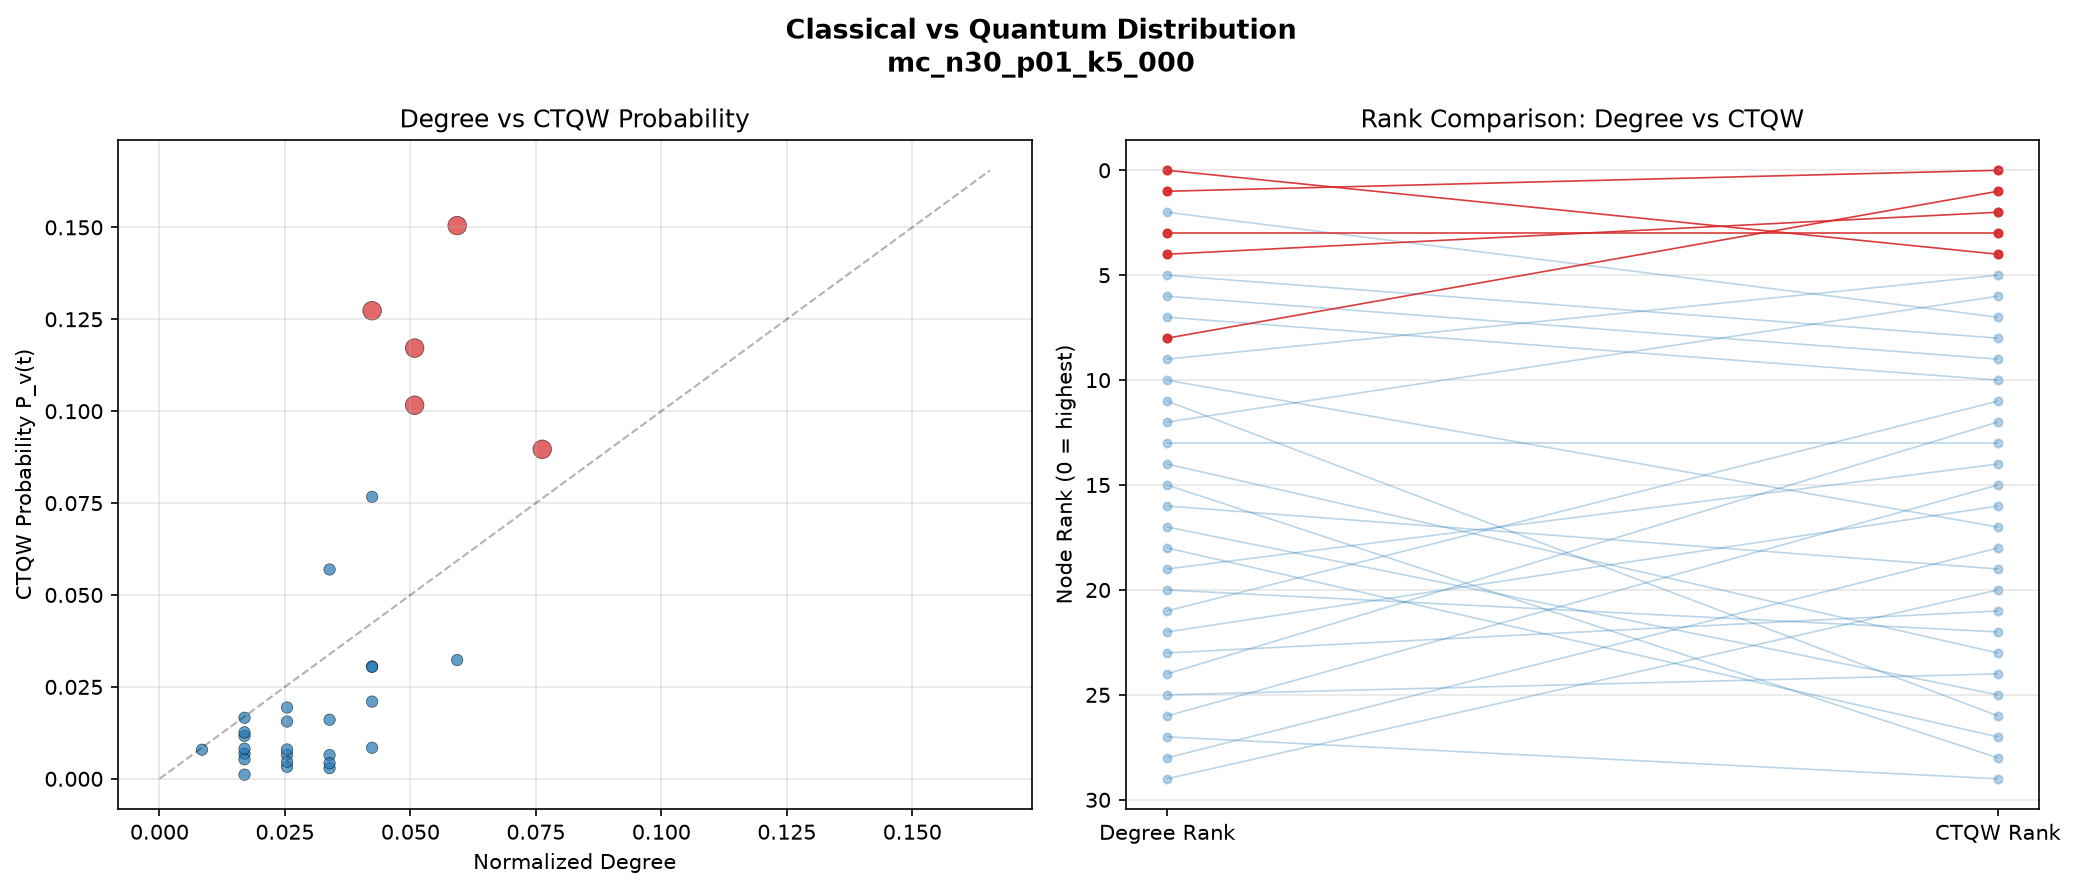
\includegraphics[width=8.4cm]{figures/exp1_ctqw_compare.png}
\caption{度数与 CTQW 概率的对比（$n=30$，植入 5-团）。红色团节点的 CTQW 概率均“超出”其度数信号，位于 $y=x$ 对角线上方。}
\label{fig:exp1}
\end{figure}

\subsection{实验二（H2）：嵌入式量子引导贪心}
\textbf{目的}：验证假设 H2——将 CTQW 嵌入贪心迭代（每轮按当前 $S$ 重算概率并按式~\eqref{eq:score} 混合）能否提升求解质量。在 small 规模上，经典强基线 ClassicalClique 取得 $7.20$ 的平均团大小，反而高于混合方案（$\alpha{=}0.5$，$6.71$）、纯度数贪心（$6.66$）与模拟退火（$6.50$）。

$\alpha$ 参数扫描（表~\ref{tbl:alpha}）显示性能随 $\alpha$ \textbf{严格单调递减}、不存在中间最优；medium 规模上差距随规模\emph{扩大}，排除了“基线偶然偏强”的解释。组件消融（表~\ref{tbl:ablation}）表明 $R$ 评分贡献了绝大部分性能（去掉后下降约 $35\%$），种子扰动 $\lambda$ 几乎无影响（B 与 C 仅差 $0.9\%$），混合方案 D 虽显著优于纯量子 B/C（$+43\%$）但仍逊于纯经典 A（$-6.8\%$）。参数敏感性进一步显示：$\alpha\le0.25$ 在所有 $(\lambda,t)$ 下稳定找回完整 5-团，$\alpha\ge0.75$ 多数情况下崩溃到 $2$--$3$ 团。

\begin{table}[H]
\caption{实验二 $\alpha$ 参数扫描（small 规模，平均团大小）。}
\label{tbl:alpha}
\centering
\begin{tabular}{ccc}
\hline\hline
$\alpha$ & 平均团大小 & $\Delta$ vs 基线 \\
\hline
0.00（经典） & 7.20 & $+0.00$ \\
0.25 & 7.14 & $-0.06$ \\
0.50 & 6.71 & $-0.49$ \\
0.75 & 5.08 & $-2.12$ \\
1.00（纯量子） & 4.65 & $-2.55$ \\
\hline\hline
\end{tabular}
\end{table}

\begin{table}[H]
\caption{实验二组件消融（MC small，平均团大小）。}
\label{tbl:ablation}
\centering
\begin{tabular}{lcc}
\hline\hline
配置（Q：量子，R：度数，$\lambda$：扰动） & 平均团大小 & 相对基线 \\
\hline
A 纯经典（R） & 7.20 & --- \\
B 纯量子（Q，$\lambda{=}0$） & 4.71 & $-34.6\%$ \\
C 纯量子（Q，$\lambda{>}0$） & 4.65 & $-35.5\%$ \\
D 完整混合（Q+R） & 6.71 & $-6.8\%$ \\
\hline\hline
\end{tabular}
\end{table}

\textbf{机理诊断}：贪心迭代中初始态为种子集合叠加，CTQW 概率集中于“与 $S$ 强相连”的节点——\emph{而这恰是 $R$ 评分已经在寻找的目标}。两者回答同一问题，但 $Q$ 受相位干涉影响、精度低于确定的整数度数计数，混合后反而污染了 $R$ 的好决策。按 $\alpha$ 分层的召回率印证了这一点：$\alpha=0$ 时 $0.925$，$\alpha=0.5$ 时 $0.865$，$\alpha=1.0$ 时跌至 $0.556$。\textbf{结论}：嵌入式方案被经典度数评分覆盖，混合优于单一量子但未超越经典。

\subsection{实验三（H3）：外置式起点选择器}
\textbf{目的}：基于实验二的失败诊断，验证假设 H3——将 CTQW 移出贪心、置于其外部专做起点选择器是否能反超经典强基线。\textbf{保留实验一验证有效的全图均匀叠加初态}：以 $S=\varnothing$、$H=A$ 计算 CTQW 概率，取概率最高的 $K$ 个节点为种子分别做经典贪心后取最大团。对照算法 MultiStartRandom、MultiStartDegree 分别剥离“多起点本身有效”与“任意全局信号都有效”两种替代解释。medium 规模主对照（$K{=}10$，表~\ref{tbl:exp3}）中 MultiStartCTQW 以 $p<0.001$ 显著超越经典强基线，这是项目中\emph{首次}出现量子方案在严格对照下胜过强基线。不过 CTQW 与度数信号在 planted-clique 上高度相关（small $K{=}10$ 时两者 Top-$K$ 完全相同），CTQW 在该数据集上未提供度数之外的额外信息。\textbf{结论}：外置式方案成立，H3 在 medium 规模上得到支持，验证了机理诊断的方向正确。

\begin{table}[H]
\caption{实验三 medium 规模主对照（$K=10$）。}
\label{tbl:exp3}
\centering
\begin{tabular}{lccc}
\hline\hline
算法 & 平均团大小 & $\Delta$ & $p$ \\
\hline
ClassicalClique（基线） & 11.70 & --- & --- \\
MultiStartRandom & 9.91 & $-1.80$ & $<0.001$ \\
MultiStartDegree & 12.38 & $+0.68$ & $<0.001$ \\
MultiStartCTQW & 12.41 & $+0.71$ & $<0.001$ \\
\hline\hline
\end{tabular}
\end{table}

\subsection{实验四（H4）：大规模真实数据测试}
\textbf{目的}：验证假设 H4——把方法迁移到大规模图、用稀疏近似替换精确矩阵指数后，前述结论是否依然成立。精确的矩阵指数复杂度为 $O(n^3)$，在大图上不可行。为此实现两种只需稀疏矩阵-向量乘法的近似——Krylov 子空间法与 Chebyshev 多项式法，并对嵌入式与外置式两种量子引导方案，在大规模人工数据集与 DIMACS 真实数据集上做效率与准确度测试。图~\ref{fig:exp6} 给出外置式的大规模对比总览。

\begin{figure}[H]
\centering
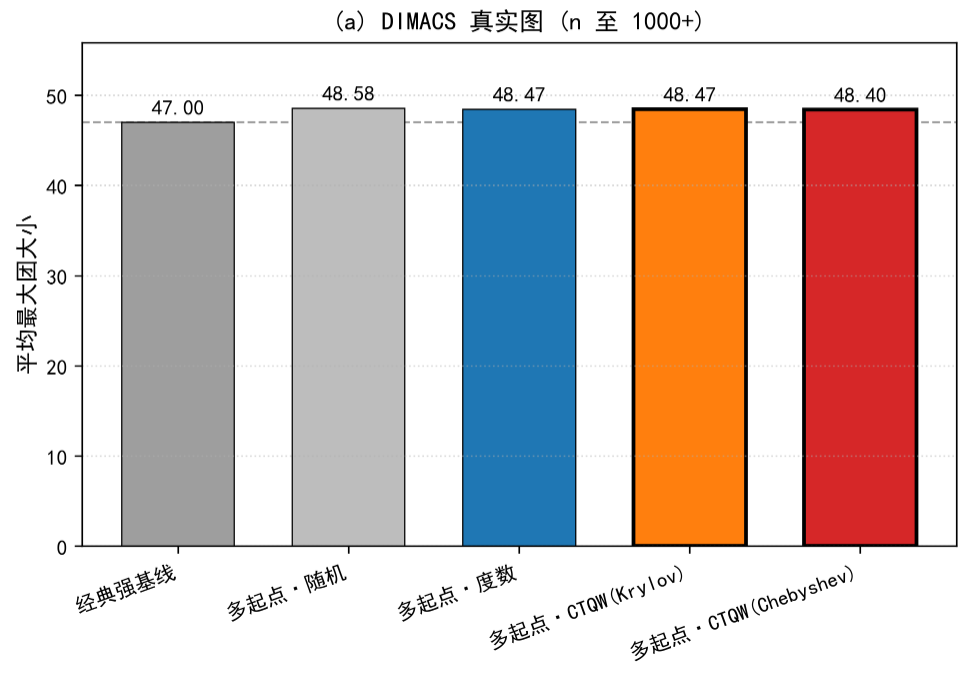
\includegraphics[width=\columnwidth]{figures/柱状图1.png}\\[2pt]
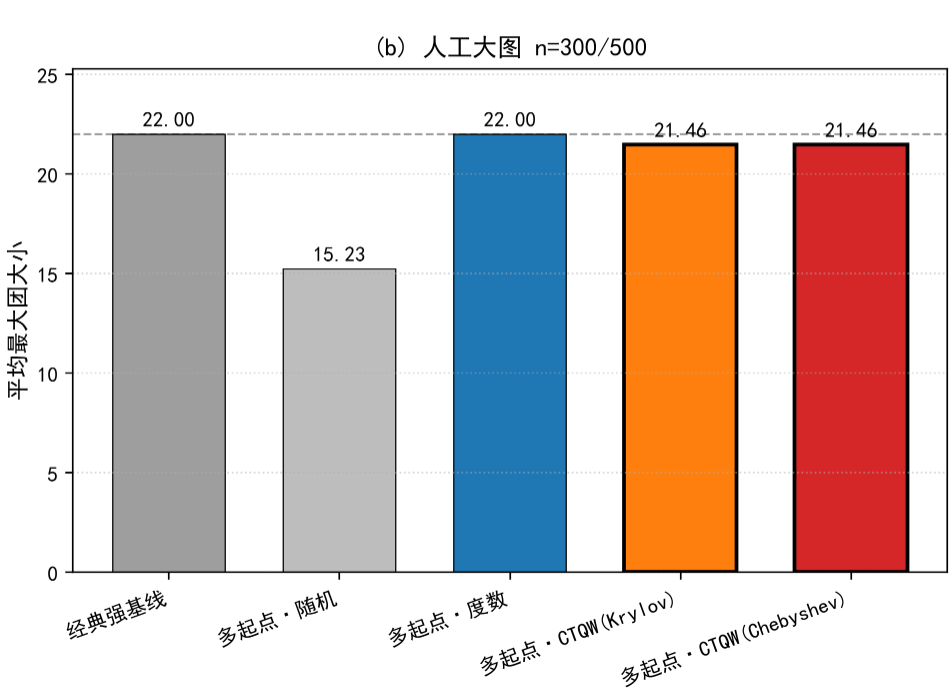
\includegraphics[width=\columnwidth]{figures/柱状图2.png}
\caption{外置式方案在大规模图上各起点选择策略的平均最大团大小。上 (a) 为 DIMACS 真实图（$n$ 至 $1000+$），下 (b) 为人工大图 $n=300/500$；虚线为经典强基线水平，橙/红为 CTQW 的 Krylov 与 Chebyshev 两种近似。两数据集上 multi-start 智能起点均逼近或超过基线，随机起点明显掉队。}
\label{fig:exp6}
\end{figure}

\textbf{嵌入式 $\times$ 人工数据集}：两种量子引导贪心与多数经典贪心一样都能精准找到最大团，而模拟退火未能精准找到；耗时方面 Chebyshev 显著高于其它算法，经典的 ClassicalDegree 与 ClassicalClique 耗时略低于 Krylov，模拟退火与 Krylov 相近。

\textbf{外置式 $\times$ 人工数据集}：随重启次数 $K$ 从 $5$ 增至 $30$，经典贪心一直精准找到大小为 $22.0$ 的最大团；Krylov 与 Chebyshev 表现一致，所找最大团从 $20.7$ 增至 $22.0$，逐渐达到经典算法水平。

\textbf{嵌入式 $\times$ DIMACS 真实数据集}：经典算法找到的最大团均大于两种量子引导贪心，其中经典 CliqueGreedy 明显最高、Chebyshev 最小；耗时方面 Chebyshev 最长且不稳定，DegGreedy 最短，CliqueGreedy 与 Krylov 居中且接近（Krylov 略快）。

\textbf{外置式 $\times$ DIMACS 真实数据集}：为减少耗时，去除耗时长且不稳定的 Chebyshev、缩减重复次数为 $1$、重启次数 $K{=}5$；虽然数据的准确性与丰富度被极大缩减，但此时 Krylov 找到的最大团大小为 $48.4$，略大于经典 Degree 的 $47.8$。推测在处理真实数据集时，由于量子游走能更好地反映图的全局拓扑结构，外置式量子引导贪心的准确度可能反超经典算法。

\section{结论与展望}

四组实验给出一致的图景：CTQW 能识别图的全局团结构（实验一）；将其嵌入贪心内部时被经典度数评分覆盖、并无优势（实验二）；改作贪心外部的起点选择器时则能显著超越经典强基线（实验三）；在大规模真实数据上，嵌入式仍无优势，外置式处理人工数据略低于经典、但外置式 Krylov 近似处理 DIMACS 真实数据的准确度有反超经典算法的趋势（实验四）。

最关键的发现是：\textbf{CTQW 的全局识别能力本身真实可靠，但其有效性高度依赖具体的使用方式}——置于贪心外部并保留全图均匀叠加初态时能发挥优势，嵌入贪心内部、改用种子集合叠加初态时则被度数覆盖。这两种用法对应 CTQW 的两种不同物理模式：全局拓扑识别与局部种子扩散。综合效率与准确度，嵌入式量子引导贪心相对经典并无优势；外置式 Krylov 近似在真实数据集上的准确度可能略高于经典算法，是更有前景的方向。后续工作包括去均匀基线的 $Q$ 评分、以 $Q$ 作二级排序的打破平局策略、多时间平均评分，以及在更多真实图族上进一步解耦 CTQW 与度数信号。

\appendix
\section{代码清单与复现说明}

完整代码见 GitHub 仓库 \texttt{https://github.com/Pease698/ZJUQI-QuantumWalk}，核心依赖为开源软件 SciPy~\cite{scipy2020} 与 NetworkX~\cite{networkx2008}。各实验复现入口为 \texttt{experiments/exp1\_*.py} 至 \texttt{exp6\_*.py}；近似方法位于 \texttt{src/ctqw\_evolution.py}。下面给出 CTQW 单轮概率计算的核心代码：

\begin{verbatim}
import numpy as np
import scipy.linalg as la

def ctqw_probs(adjacency, S, lam, t,
               init_method="uniform"):
    # H = A + lam * sum_{u in S} |u><u|
    H = construct_hamiltonian(adjacency, S, lam)
    psi0 = build_initial_state(
        len(adjacency), S, adjacency,
        init_method)
    U = la.expm(-1j * H * t)   # evolution
    psi_t = U @ psi0           # propagate
    return np.abs(psi_t) ** 2  # P_v
\end{verbatim}

\begin{thebibliography}{99}

\bibitem{farhi1998}
E. Farhi and S. Gutmann, Quantum computation and decision trees, Phys.\ Rev.\ A \textbf{58}, 915 (1998).

\bibitem{childs02}
A. M. Childs, E. Farhi, and S. Gutmann, An example of the difference between quantum and classical random walks, Quantum Inf.\ Process.\ \textbf{1}, 35 (2002).

\bibitem{kempe2003}
J. Kempe, Quantum random walks: an introductory overview, Contemp.\ Phys.\ \textbf{44}, 307 (2003).

\bibitem{venegas2012}
S. E. Venegas-Andraca, Quantum walks: a comprehensive review, Quantum Inf.\ Process.\ \textbf{11}, 1015 (2012).

\bibitem{childs2009}
A. M. Childs, Universal computation by quantum walk, Phys.\ Rev.\ Lett.\ \textbf{102}, 180501 (2009).

\bibitem{kirkpatrick1983}
S. Kirkpatrick, C. D. Gelatt, and M. P. Vecchi, Optimization by simulated annealing, Science \textbf{220}, 671 (1983).

\bibitem{pardalos1994}
P. M. Pardalos and J. Xue, The maximum clique problem, J.\ Global Optim.\ \textbf{4}, 301 (1994).

\bibitem{dimacs1996}
D. S. Johnson and M. A. Trick (eds.), \textit{Cliques, Coloring, and Satisfiability: Second DIMACS Implementation Challenge} (American Mathematical Society, 1996).

\bibitem{scipy2020}
P. Virtanen \textit{et al.}, SciPy 1.0: fundamental algorithms for scientific computing in Python, Nat.\ Methods \textbf{17}, 261 (2020).

\bibitem{networkx2008}
A. A. Hagberg, D. A. Schult, and P. J. Swart, Exploring network structure, dynamics, and function using NetworkX, in \textit{Proc.\ 7th Python in Science Conf.}\ (2008), pp.\ 11--15.

\end{thebibliography}

\end{document}
